\documentclass{article}
\usepackage{epsf}\usepackage{here}\usepackage{latexsym}
\usepackage{graphicx}
\usepackage{graphicx}
\oddsidemargin 0.25in \evensidemargin 0.25in
\topmargin 0.0in
\textwidth 6.5in \textheight 8.5in
\headheight 0.18in \footskip 0.16in
\leftmargin -0.5in \rightmargin -0.5in

%
% KEYWORD
%
\newcommand{\keywordtable}[1]{
        \sloppy
        \hyphenation{ca-pac-i-t-an-ce}
        \begin{center}
    \sf
        \begin{tabular}[t]
        {|p{0.58in}|p{3.07in}|p{0.55in}|p{0.60in}|}
        \hline
        \multicolumn{1}{|c}{\bf Name} &
        \multicolumn{1}{|c}{\parbox{2.77in}{\bf Description}}  &
        \multicolumn{1}{|c}{\bf Units} &
        \multicolumn{1}{|c|}{\bf Default} \X
        #1
        \end{tabular}
        \end{center}
    }

\newcommand{\keywordtwotable}[2]{
        \sloppy
        \hyphenation{ca-pac-i-t-an-ce}
        \begin{center}
    \sf
        \begin{tabular}[t]
        {|p{0.58in}|p{2.38in}|p{0.55in}|p{0.60in}|p{0.53in}|}
        \hline
        \multicolumn{1}{|c}{\bf Name} &
        \multicolumn{1}{|c}{\parbox{2.20in}{\bf Description}}  &
        \multicolumn{1}{|c}{\bf Units} &
        \multicolumn{1}{|c}{\bf Default} &
        \multicolumn{1}{|c|}{\bf #1} \X
        #2
        \end{tabular}
        \end{center}
    }

\newcommand{\kw}[2]{
     \samepage{
     \noindent {\sl #1} \vspace{-0.5in} \\
     \keywordtable{#2} }}

\newcommand{\kwtwo}[3]{
     \samepage{
     \noindent {\sl #1} \vspace{-0.4in} \\
     \keywordtwotable{#2}{#3} }}

\newcommand{\keyword}[1]{\kw{Keywords:}{#1}}
\newcommand{\keywordtwo}[2]{\kwtwo{Keywords:}{#1}{#2}}
\newcommand{\modelkeyword}[1]{\kw{Model Keywords}{#1}}
\newcommand{\modelkeywordtwo}[2]{\kwtwo{Model Keywords}{#1}{#2}}

\newcommand{\myline}{\\[-0.1in]
\noindent \rule{\textwidth}{0.01in} \newline}

\newcommand{\myThickLine}{\\[-0.1in]
\noindent \rule{\textwidth}{0.02in} \newline}


% FORM
\newcommand{\form}[1]{\samepage{\noindent
 {\sl Form} \myline
% \hspace*{\fill} % For some reason \fill = 0 when \pspiceform{} is used?
\offset
\it  \offsetparbox{#1}}
\\[0.1in]}

% ELEMENT FORM
\newcommand{\elementform}[1]{\samepage{\noindent
 {\sl Element Form} \myline
% \hspace*{\fill} % For some reason \fill = 0 when \pspiceform{} is used?
\offset
\it  \offsetparbox{#1}}
\\[0.1in]}

% MODEL FORM
\newcommand{\modelform}[1]{\samepage{\noindent
 {\sl Model Form} \myline
% \hspace*{\fill} % For some reason \fill = 0 when \pspiceform{} is used?
\offset
\it  \offsetparbox{#1}}
\\[0.1in]}

% LIMITS
\newcommand{\mylimits}[1]{\samepage{\noindent
 {\sl Limits} \myline
 \hspace*{\fill} \it  \offsetparbox{#1}}
 \vshift}

% EXAMPLE
\newcommand{\example}[1]{\samepage{\noindent
{\sl Example} \myline
\offset \tt  \offsetparbox{#1}}
 \vshift}

% PSPICE88 EXAMPLE
\newcommand{\pspiceexample}[1]{\samepage{\noindent
{\sl \pspice\ Example} \myline
\offset \tt  \offsetparbox{#1}}
 \vshift}

% MODEL TYPES
\newcommand{\modeltype}[1]{\samepage{\noindent
{\sl Model Type} \myline
 \hspace*{\fill} \tt \offsetparbox{#1}}
 \\[0.1in]}

% MODEL TYPES
\newcommand{\modeltypes}[1]{\samepage{\noindent
{\sl Model Types:} \myline
 \hspace*{\fill} \tt \offsetparbox{\tt #1}}
 \vshift}

% OFFSET ENUMERATE
\newcommand{\offsetenumerate}[1]{
     \offset \hspace*{-0.1in} {\begin{enumerate} #1 \end{enumerate}}}

% NOTE
\newcommand{\note}[1]{
\vshift\samepage{\noindent {\sl Note}\myline\vspace{-0.24in}}
 \offsetenumerate{#1} }

% SPECIAL NOTE
\newcommand{\specialnote}[2]{
\vshift\samepage{\noindent {\sl #1}\myline\vspace{-0.24in}}\\#2}

\newcommand{\dc}{\mbox{\tt DC}}
\newcommand{\ac}{\mbox{\tt AC}}
\newcommand{\SPICE}{\mbox{\tt SPICE}}
\newcommand{\m}[1]{{\bf #1}}                           % matrix command  \m{}

% ////// Changing nodes to terminals///////
% print terminals in \tt and enclose in a circle use outside
\newcommand{\terminal}[1]{\: \mbox{\tt #1} \!\!\!\! \bigcirc }
%
% set up environment for example
%
\newcounter{excount}
\newcounter{dummy}
\newenvironment{eg}{\vspace{0.1in}\noindent\rule{\textwidth}{.5mm}
   \begin{list}
   {{\addtocounter{excount}{1}
   \em Example\/ \arabic{chapter}.\arabic{excount}\/}:}
   {\usecounter{dummy}
   \setlength{\rightmargin}{\leftmargin}}
   }{\end{list} \rule{\textwidth}{.5mm}\vspace{0.1in}}
%
% set up environment for block
% currently this draws a horizontal line at the start of block and another
% at the end of block.
%
\newenvironment{block}{\vspace{0.1in}\noindent\rule{\textwidth}{.5mm}
   }{\rule{\textwidth}{.5mm}\vspace{0.1in}}
%


%
% set up wide descriptive list
%
\newenvironment{widelist}
    {\begin{list}{}{\setlength{\rightmargin}{0in} \setlength{\itemsep}{0.1in}
    \setlength{\labelwidth}{0.95in} \setlength{\labelsep}{0.1in}
\setlength{\listparindent}{0in} \setlength{\parsep}{0in}
    \setlength{\leftmargin}{1.0in}}
    }{\end{list}}

\newcommand{\STAR}{\hspace*{\fill} * \hspace*{\fill}}

\newcommand{\sym}[1]{\hspace*{\fill} ($#1$)}

\newcommand{\optionitem}[2]{
\item[{\tt #1}{#2}]\label{.OPTION#1}\index{.OPTIONS, #1}\index{#1}}

\newcommand{\error}[1]{\vspace{0.1in}\noindent{\tt #1}\\}


\begin{document}
\noindent{\LARGE \textbf{Multi-port element defined by Foster's
\\canonical form} \hspace{\fill}\textbf{nportFoster}}
\hrulefill\linethickness{0.5mm}\line(1,0){425} \normalsize
\newline
% form for \FDA
%\linethickness{0.5mm} \line(1,0){425}
%\newline
\textit{Form:}
%\newline
$\tt nportFoster$:$\langle \tt{instance\ name}\rangle$ $n_1\ n_2\
\cdots$ $\langle \tt{parameter\ list}\rangle$
\newline
\begin{tabular}{r l}
$n_1$, $n_2$ $\cdots$ & are the element nodes. \\
\end{tabular}
% Parameter list
\newline
\textit{Parameters:}
\begin{table}[H]
\begin{tabular}{|c|c|c|c|}
\hline
Parameter&Type&Default value&Required?\\
\hline
filename: File containing the & STRING & n/a & yes\\
pole-residue data. & & & \\
\hline
ports: Number of ports & INTEGER & n/a & yes\\
\hline
poles1: Number of poles & INTEGER & n/a & yes\\
\hline
poles2: Number of poles & INTEGER & n/a & yes\\
\par
\hline
\end{tabular}
\end{table}
% example in \FDA
\noindent\linethickness{0.5mm}\line(1,0){425}
\newline
\textit{Example:}
\newline
\texttt{fosternport:\ f1\ 1\ "0"\ 2\ "0"\ 3\ "0"\ 4\ "0"\ 5\
"0"\ 6\ "0"\\
filename = "testfosternport.yp" ports="6" poles1="36" poles2="36"\\
.ref "0"}


\textbf{DESCRIPTION:}

\begin{itemize}
\item The element is implemented as a Linear Voltage Controlled Current Source
\item The method followed for this implementation is the \textit{``Pole -- Residual'' }method as it gives better numerical stability
\item This is a N-Port generalization and so it would work for any number of ports and poles
\end{itemize}

\textbf{TECHNICAL APPROACH :}

\begin{itemize}
\item Each element in the multi -- port Admittance matrix is described by its own rational function in the pole -- residue format
\item In this format different elements in the Admittance matrix may have different poles(meaning values for the poles)
\item But all the elements in the Admittance matrix must have the same number of poles
\item The representation made use of here is the Foster's Canonical representation
\item Foster's Canonical representation is given as :
\end{itemize}
\[
H(s)=\sum\limits_{j=1}^m {\frac{k_j }{s-p_j }} +\left( {\sum\limits_{j=1}^m
{\frac{k_j }{s-b_j }+\frac{a_j^\ast }{s-b_j^\ast }} } \right)
\]
Here ${k_j } \mathord{\left/ {\vphantom {{k_j } {\left( {s-p_j } \right)}}}
\right. \kern-\nulldelimiterspace} {\left( {s-p_j } \right)}$ represents the
real pole and ${a_j } \mathord{\left/ {\vphantom {{a_j } {\left( {s-b_j }
\right)}}} \right. \kern-\nulldelimiterspace} {\left( {s-b_j } \right)}$
plus ${a_j } \mathord{\left/ {\vphantom {{a_j } {\left( {s-b_j } \right)}}}
\right. \kern-\nulldelimiterspace} {\left( {s-b_j } \right)}$ together
represents the complex conjugate pairs

\begin{itemize}
\item Frequency domain analysis is very straight forward as the given pole -- residue data set is just plotted
\item Time domain analysis involves complexity in the calculation of the Modified Nodal Admittance Matrix as it involves the derivatives
\end{itemize}

\textbf{FILLING OF THE MODIFIED NODAL ADMITTANCE MATRIX :}

\begin{itemize}
\item Number of ports and number of poles (also the data file set) are taken as the input parameters necessary for the netlist
\item Suppose we have a 2 -- port network, then we should have 4 instances of the given element(FosterNPort), that is, if Y(s) = [H$_{11}$(s) H$_{12}$(s) ; H$_{21}$(s) H$_{22}$(s)], then each H$_{ii}$(s) could be represented by this element
\item In the data set, there is a real pole -- residue expression and a complex pole -- residue expression. The complex pole -- residue expression is converted to real pole -- residue format and then plugged in the matrix. In this way the element is created for each transfer function and connected in the circuitry.
\item There is a function called the \textit{``fillMNAM''} function which fills the modified nodal admittance matrix with the calculated transfer function values. A loop is put with respect to the \textit{``fillMNAM''} function. For each iteration of the loop, the previous calculation is done and plugged for each `element'
\item Suppose if we have a 6 -- port network then there can be any number of terminals between 7 and 12. In order to reduce the complexity of local reference nodes, we take half of the terminals as just one reference for all the ports. So here I have 7 terminals from 0 to 6, with the 6$^{th}$ terminal taken as the reference
\item In the frequency domain, the transfer function matrix is of the form :
\end{itemize}


\centerline{\includegraphics{foster0.eps}}

\begin{itemize}
\item Each i[][] and j[][] contains 36 elements(as the given data set has 36*36 real
\end{itemize}
Poles and complex poles each)

\begin{itemize}
\item And each element in i[][] is represented by a setQuad function given by :
\end{itemize}
mnam -$>$ setQuad ( getTerminal(i)-$>$getRC(),

getTerminal(ports)-$>$getRC(),

getTerminal(j)-$>$getRC(),

getTerminal(ports)-$>$getRC(),g)

wherein each element has the Admittance matrix stamp which is [g -g; -g g]



\textbf{REPRESENTATION OF FOSTER'S FORM IN THE NETLIST :}

\textbf{$<$}filename$>$:$<$name of the element$> \quad <$terminal numbers$>$
$<$filename = $> \quad <$ports = $>$

$<$poles = $>$

For example:

NPortFoster:f1 1 2 3 4 5 6 0 filename = `transimtest.yp' ports = 6 poles =
36

\noindent\textbf{RESULTS :}

\begin{enumerate}
\item \textbf{2 -- Port network using 4 instances of the element:}
\end{enumerate}

\noindent\textbf{CIRCUIT :}

\begin{figure}
\centerline{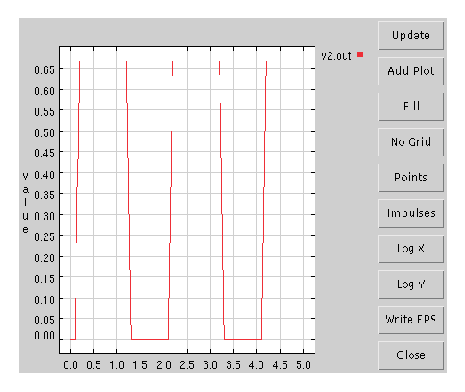
\includegraphics{foster1.eps}}
\label{fig1}
\end{figure}
\begin{figure}
\centerline{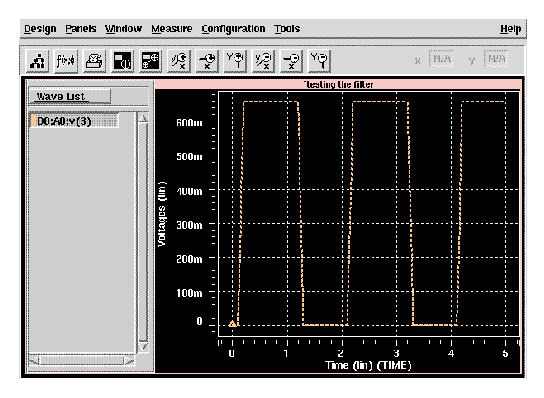
\includegraphics{foster2.eps}}
\label{fig2}
\end{figure}
\begin{figure}
\centerline{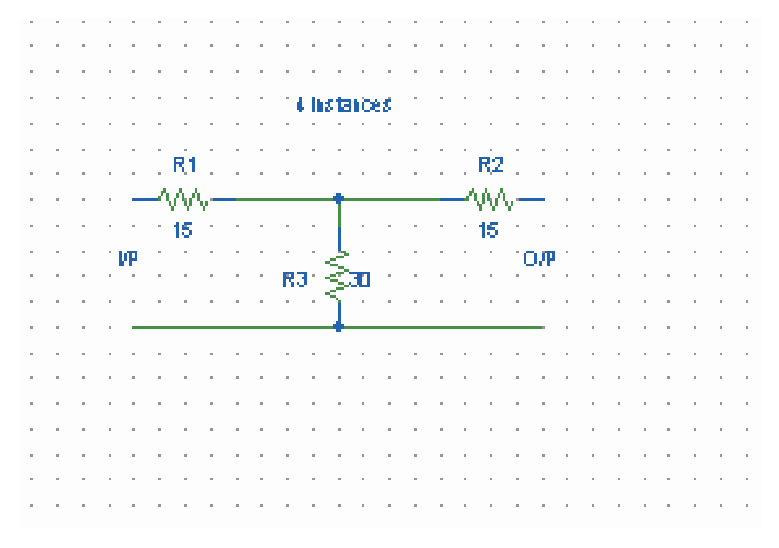
\includegraphics{foster3.eps}}
\label{fig3}
\end{figure}


\linethickness{0.5mm} \line(1,0){425}
\newline
\textit{Notes:}\\
There is no equivalent SPICE element.\\
\linethickness{0.5mm} \line(1,0){425}
\newline
\textit{Version:}\\
2002.06.01 \\
% Credits
\linethickness{0.5mm} \line(1,0){425}
\newline
\textit{Credits:}\\
\begin{tabular}{l l l l}
Name & Affiliation & Date & Links \\
Ramya Mohan & NC State University & June 2002 & \epsfxsize=1in\epsfbox{logo.eps}  \\
ramya@ieee.org & & & www.ncsu.edu    \\
\end{tabular}
\end{document}
